\textnormal{This project will use multiple technologies for both the front-end and the back-end. For the back end, we plan to use an SQL database to store the Course, Professor, and TA data. Java servlets will be used for for code execution. For the front-end, we plan on using Angular and Javascript for the layout and D3.js for the visual representation of the 3D matching. We may use jQuery for SQL query manipulation that will serve input to the 3D matching approximation algorithm.}

\begin{figure}
	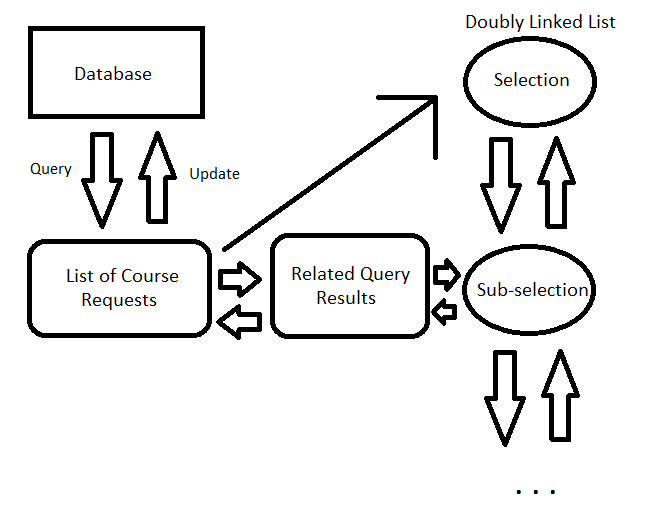
\includegraphics[width=\linewidth]{Data_Structures.png}
	\caption{Internal Data Structures}
	\label{fig:fig1}
\end{figure}

As shown in Figure \ref{fig:fig1}, the back-end operations will be driven by queries to the MySQL database as well as the 3D matching approximation algorithm. The results of the matching algorithm will be fed into the D3.js API that will generate a visual representation of the matching. The user will be able to visualize and manipulate the 3D matching to generate different instances (i.e. solutions) of the matching. When the user selects certain nodes on the interface, such as a specific student or class, those nodes will reference a linked list of triples for which the node belongs allowing the user to quickly visualize local interaction between nodes. The current state of the instance of the 3D matching representation will be stored in a doubly linked list that will allow for progression and regression of the visual interface.  Using a linked list will allow the user to navigate through different instances (solutions) quickly without having to re-run the approximation algorithm.
\\\\